\documentclass[12pt,a4paper,openany]{scrbook}
\usepackage[left=3.00cm, right=2.00cm, top=2.00cm, bottom=3.00cm]{geometry}
\usepackage[latin1]{inputenc}
\usepackage{longtable}
\usepackage{array}
\usepackage[bahasa]{babel}
\usepackage{indentfirst}
\usepackage{palatino}
\usepackage{microtype}
\usepackage{floatflt}
\usepackage{graphicx}
\usepackage{multirow}

\makeatletter
%==========redefine chapter and section
\def\ps@chapterheading{%
	\let\@evenhead\@empty\let\@oddhead\@empty
	\def\@oddfoot{\hfil\thepage\hfil}%
	\def\@evenfoot{\hfil\thepage\hfil}
}
\setcounter{secnumdepth}{2}
\renewcommand \thepart {\@Roman\c@part}
\renewcommand \thechapter {\@Roman\c@chapter}
%\renewcommand \thesection {\@arabic\c@section.}
\renewcommand \thesection {\@arabic\c@chapter.\@arabic\c@section}
%\renewcommand\thesubsection {\@alph\c@subsection.}
\renewcommand\thesubsection {\@arabic\c@chapter.\@arabic\c@section.\@arabic\c@subsection}
%\renewcommand\thesubsubsection{\@roman\c@subsubsection.}
%\renewcommand\thesubsubsection{}
\renewcommand\appendix{\par
	\setcounter{chapter}{0}%
	\setcounter{section}{0}%
	\gdef\@chapapp{\appendixname}%
	\gdef\thechapter{\@Alph\c@chapter}}
\renewcommand{\chapter}{\clearpage\thispagestyle{chapterheading}%
	\global\@topnum\z@ %Prevents figures from going at top of page
	\@afterindenttrue %Indent the 1st paragraph
	\secdef\@chapter\@schapter}
\renewcommand{\@makechapterhead}[1]{%
	{\parindent \z@ \centering \normalfont
		\ifnum \c@secnumdepth >\m@ne
		\large\bfseries \@chapapp\space \thechapter
		\par\nobreak
		\vskip 5\p@
		\fi
		\interlinepenalty\@M
		\large \bfseries #1\par\nobreak
		\vskip 20\p@
}}
\renewcommand{\@makeschapterhead}[1]{%
	{\parindent \z@ \centering \normalfont
		\interlinepenalty\@M \large \bfseries #1\par\nobreak \vskip 20\p@ }}
%\renewcommand{\section}{\@startsection {section}{1}{\z@}%
%                                   {-3.5ex \@plus -1ex \@minus -.2ex}%
%                                   {2.3ex \@plus.2ex}%
%                                   {\normalfont\normalsize\bfseries\centering}}
\renewcommand{\section}{\@startsection {section}{1}{\z@}%
	{-3.5ex \@plus -1ex \@minus -.2ex}%
	{2.3ex \@plus.2ex}%
	{\normalfont\normalsize\bfseries}}
\renewcommand{\subsection}{\@startsection{subsection}{2}{\z@}%
	{-3.25ex\@plus -1ex \@minus -.2ex}%
	{1.5ex \@plus .2ex}%
	{\normalfont\normalsize\bfseries}}
%\renewcommand{\subsubsection}{\@startsection{subsubsection}{3}{\parindent}%
%                                    {3.25ex \@plus1ex \@minus.2ex}%
%                                    {-1em}%
%                                    {\normalfont\normalsize\bfseries}}
\renewcommand{\subsubsection}{\@startsection{subsubsection}{3}{\z@}%
	{3.25ex \@plus1ex \@minus.2ex}%
	{-1em}%
	{\normalfont\normalsize\bfseries}}
\renewcommand{\paragraph}{\subparagraph}

\@addtoreset {equation}{chapter}
\renewcommand\theequation
{\ifnum \c@chapter>\z@ \@arabic\c@chapter.\fi \@arabic\c@equation}
\renewcommand \thefigure
{\ifnum \c@chapter>\z@ \@arabic\c@chapter.\fi \@arabic\c@figure}
\renewcommand \thetable
{\ifnum \c@chapter>\z@ \@arabic\c@chapter.\fi \@arabic\c@table}

%------------------------------------------------------------
%Redefine caption names
%------------------------------------------------------------
\def\captionsbahasa{%
	\def\prefacename{PRAKATA}%
	\def\contentsname{DAFTAR ISI}%
	\def\listfigurename{DAFTAR GAMBAR}%
	\def\listtablename{DAFTAR TABEL}%
	\def\listappendixname{DAFTAR LAMPIRAN}%
	\def\nomenclaturename{DAFTAR LAMBANG DAN SINGKATAN}%
	\def\abstractname{INTISARI}%
	\def\partname{BAGIAN}%
	\def\chaptername{BAB}%
	\def\appendixname{LAMPIRAN}%
	\def\refname{DAFTAR PUSTAKA}%
	\def\bibname{DAFTAR PUSTAKA}%
	\def\indexname{Indek}%
	\def\figurename{Gambar}%
	\def\tablename{Tabel}%
	\def\pagename{Halaman}%
}

\makeatother

\newcounter{nourut}
\newcommand{\nexturut}{%
	\stepcounter{nourut}
	\arabic{nourut}}


%=========== identity==============
\newcommand{\lingkungan}{St. Theresia Pugeran}
\newcommand{\wilayah}{St. Yohanes Don Bosco}
\newcommand{\tahun}{2016}
\newcolumntype{L}[1]{>{\raggedright\arraybackslash}p{#1}}
\newcolumntype{C}[1]{>{\centering\arraybackslash}p{#1}}
\newcolumntype{R}[1]{>{\raggedleft\arraybackslash}p{#1}}
\uchyph=1
\hyphenation{YOG-YA-KAR-TA Sle-man}

\title{STATISTIK LINGKUNGAN\\\lingkungan\\WILAYAH \wilayah\\~\\~ STASI BUNDA MARIA MAGUWO}
\author{Dewan Stasi Maguwo}
\date{\tahun}

\begin{document}
\maketitle

\chapter{Sejarah Lingkungan}
\section{Lahirnya Lingkungan St. Theresia Kanak-kanak Yesus}
Pada akhir tahun 2013 yaitu pada bulan September, semua lingkungan di Stasi Maguwo 
diharapkan melakukan pemilihan pengurus baru. Sesuai dengan mekanisme pemilihan dari paroki, 
maka dilakukanlah pemilihan pengurus baru yang diketuai oleh Andreas Keso Muda.
Pemilihan berhasil memilih Anton Supriyana sebagai ketua baru. Beliau ini adalah warga baru namun stok lama. Beliau sudah lama berkecimpung di dewan paroki Pringwulung, tempat tinggal beliau sebelumnya.

\begin{floatingfigure}[l]{2cm}
	\begin{center}
		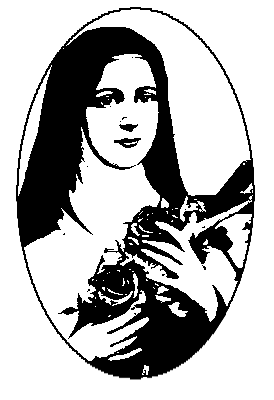
\includegraphics[scale=1]{theresia-logo.png}
	\end{center}
\end{floatingfigure}
Namun karena lingkungan Petrus dirasa terlalu banyak anggotanya, maka atas prakarsa beberapa umat, lingkungan ini diusulkan mekar menjadi 3 dan disetujui oleh umat maupun Dewan Stasi. 

Lingkungan St. Petrus kemudian mekar menjadi Lingkungan Petrus meliputi Kembang, Nanggulan, dan Tobong; Lingkungan St. Monica meliputi Maguwo, Sanggrahan, dan Karangnongko; Lingkungan St. Theresia meliputi Pugeran dan Sombomerten. 


\vspace{0.5cm}


\section{Umat St. Theresia}
Lingkungan St. Theresia mencakup 26 keluarga dengan 82 umat dengan perincian 35 laki-laki dan 47 perempuan. Namun demikian ada beberapa mahasiswa yang terlibat aktif dalam kegiatan-kegiatan lingkungan dan tidak tercatat dengan pasti karena mobilitasnya yang tinggi.

\section{Inventaris Peralatan Misa}
Sejak awal lahirnya lingkungan St. Theresia, umat sudah berkomitmen agar lingkungan mempunyai peralatan misa. Beberapa upaya yang dilakukan adalah pengumpulan data melalui tabungan receh, sumbangan sukarela, dan juga donatur dari luar. Puji syukur kepada Allah bahwa usaha-usaha tersebut banyak membuahkan hasil. Donatur dari luar, berkat ketekunan dari Bapak KRA YP Sunaryo Prononagoro mendapat banyak peralatan misa. 

Peralatan misa yang dimiliki lingkungan antara lain:
\begin{itemize}
\item peralatan altar: salib kuningan dan kayu,
korporal,
purivicatorium,
taplak,
piala,
sibori,
piksis,
patena,
aspergil,
wirug,
krincingan,
tempat lilin besar \& kecil,
patung Bunda Maria,
nampan, ampul,
tempat minyak suci.
\item pakaian liturgi: kasula,
stola,
superpli,
gaun,
kerah lebar,
singel,
alba,
samir
\item buku: buku tpe,
buku liturgi orang sakit,
mazmur tanggapan, sakramen pemberkatan,
aneka ibadat kristiani, teks doa rosario,
puji syukur, teks doa rosario bahasa Jawa.
\item elektronik: ht, \textit{wireless microphone \& speaker}, LCD projector.
\end{itemize} 

Perlu diketahui bahwa patung Bunda Maria Lourdes yang besar adalah sumbangan dari Bapak KRA YP Sunaryo Prononagoro.




\section[Pengurus]{Pengurus lingkungan}

\subsection{Periode 2014 -- 2016}

%\footnotesize 
\begin{center}
SUSUNAN PENGURUS LINGKUNGAN SANTA THERESIA 
\par
PERODE TAHUN 2014 -- 2016
\end{center}

\begin{longtable}{p{0.5cm}p{4cm}p{5cm}p{4cm}}
\multicolumn{2}{l}{Ketua I}&Antonius Supriyana &+6285 865 355 895\\
\multicolumn{2}{l}{Ketua II}&FX. Sularto &+6281 314 190 698\\
\multicolumn{2}{l}{Sekretaris I}&Anastasi Bare &+6285 643 173 281\\
\multicolumn{2}{l}{Sekretaris II}&FX. Ari Wibowo Sudaryanto&+6285 8633 5678\\
\multicolumn{2}{l}{Bendahara I}&Theresia Prima Ari Setiyani&+6285 6288 6539\\
\multicolumn{2}{l}{Bendahara II}&Agnes Sukarmi&+6281 328 795 814\\

\setcounter{nourut}{0}\\
\multicolumn{2}{l}{\textit{\textbf{Tim Kerja Liturgi}}}&&\\
&Koordinator&Yohanes Suyanto &+6285 6286 9037\\
\nexturut&Misa/Peribadatan/Doa Lingk &M.Th. Nanik Ismarjati&+6281 5686 1272\\
\nexturut&Koor&Maria Sode Muda&+6281 392 842 606\\
&&Andreas Keso Muda&+6281 328 692 102\\

\setcounter{nourut}{0}\\
\multicolumn{2}{l}{\textit{\textbf{Tim Kerja Pewartaan}}}&Neo Suradi&+6281 578 115 615\\

\setcounter{nourut}{0}\\
\multicolumn{2}{l}{\textit{\textbf{Tim Kerja Kemasyarakatan}}}&&\\
&Koordinator&Cornelius Triyono &+6281 578 179 267\\
\nexturut&Tabungan Cinta Kasih (TCK)&Kristina Tri Tutwuri &+6281 2275 2803\\
\nexturut&Prolenan&A. Sri Supriyati &+6281 328 450 101\\
\nexturut&Pangruktilaya&Th. Suci Wahyuningsih&+6281 5792 7488 \\
&&M. Th. Nanik Ismarjati&+6281 5686 1272\\
\nexturut&PSE&A. Sri Supriyati&+6281 328 450 101\\
\nexturut&Majalah Paroki/Lingkungan&OMK Lingkungan&\\

\setcounter{nourut}{0}\\
\multicolumn{2}{l}{\textit{\textbf{Tim Kerja Paguyuban}}}&&\\
&Koordinator&Ketua II&\\
\nexturut&Pag. Ibu-ibu Lingkungan&A. Hedwig Djuwarni&+6281 578 898 484\\
&&M.Goretti Budi Hartati&+6285 878 241 474\\
\nexturut&Pag. OMK Lingkungan&Stefanus Pratama Krisna Bayu Aji&\\
\nexturut&Pendamping OMK Lingk.&Neo Suradi&+6281 578 115 615\\

\setcounter{nourut}{0}\\
\multicolumn{2}{l}{\textit{\textbf{Tim Kerja Rumah Tangga}}}&&\\
\nexturut&Paramenta&Yohanes Suyanto&+6285 6286 9037\\
\nexturut&Tata Bunga&C. Prihatiningtyas S.&+6287 838 452 319\\
&&M.M.S.U.Chrissumiwi&+6281 392 301 293\\


\setcounter{nourut}{0}\\
\multicolumn{2}{l}{\textit{\textbf{Tim Kerja Humas}}}&&\\
&Koordinator&Sekretaris I&\\
\nexturut&Pugeran Utara &Kristina Tri Tutwuri &+6281 2275 2803\\
\nexturut&Pugeran Selatan&Lusia Titisari&+6283 867 812 334\\
\nexturut&Sombomerten+Pugeran Timur&Herminigilda A. Wulandari&+6287 843 023 654\\
\end{longtable}

\subsection{Periode 2017 -- 2019}

\begin{center}
	SUSUNAN PENGURUS LINGKUNGAN SANTA THERESIA 
	\par
	PERIODE TAHUN 2017 -- 2019
\end{center}
%\footnotesize 
\begin{longtable}{p{0.5cm}p{4cm}p{5cm}p{4cm}}
	\multicolumn{2}{l}{Ketua I}&Antonius Supriyana &+6285 865 355 895\\
	\multicolumn{2}{l}{Ketua II}&FX. Sularto &+6281 314 190 698\\
	\multicolumn{2}{l}{Sekretaris I}&M.M.S.U. Chrissumiwi &+6281 392 301 293\\
	\multicolumn{2}{l}{Bendahara I}&Theresia Prima Ari Setiyani&+6285 6288 6539\\
	\multicolumn{2}{l}{Bendahara II}&Agnes Sukarmi&+6281 328 795 814\\
	
	\setcounter{nourut}{0}\\
	\multicolumn{2}{l}{\textit{\textbf{Tim Kerja Liturgi}}}&&\\
	&Koordinator&Yohanes Suyanto &+6285 6286 9037\\
	\nexturut&Misa/Peribadatan/Doa Lingkungan &M.Th. Nanik Ismarjati&+6281 5686 1272\\
	\nexturut&Koor&Maria Sode Muda&+6281 392 842 606\\
	&&Valentina Isti Rudati&+6281 328 692 102\\
	
	\setcounter{nourut}{0}\\
	\multicolumn{2}{l}{\textit{\textbf{Tim Kerja Pewartaan}}}&Neo Suradi&+6281 578 115 615\\
	
	\setcounter{nourut}{0}\\
	\multicolumn{2}{l}{\textit{\textbf{Tim Kerja Kemasyarakatan}}}&&\\
	&Koordinator&Cornelius Triyono &+6281 578 179 267\\
	\nexturut&Tabungan Cinta Kasih (TCK)&Kristina Tri Tutwuri &+6281 2275 2803\\
	\nexturut&Prolenan&Roselina Zeli Puspitasari &\\
	\nexturut&Pangruktilaya&M. Th. Nanik Ismarjati&+6281 5686 1272\\
	&&C. Prihatiningtyas&+6287 838 4523\\
	\nexturut&PSE&Yohanes Sudarmadi&+6281 328 450 101\\
	\nexturut&Majalah Paroki/Lingkungan&OMK Lingkungan&\\
	
	\setcounter{nourut}{0}\\
	\multicolumn{2}{l}{\textit{\textbf{Bidang Paguyuban}}}&&\\
	&Koordinator&Aloysius Heru Pratomo&+6281 328 259 725\\
	\nexturut&Pag. Ibu-ibu Lingkungan&Anastasia Sri Supriyati&+62 813 2845 0101\\
	\nexturut&Pag. OMK Lingkungan&Maria Regina Tri Marieska&+62 813 9205 4103\\
	\nexturut&Pendamping OMK Lingk.&Andreas Keso Muda&+6281 328 692 102\\
	
	\setcounter{nourut}{0}\\
	\multicolumn{2}{l}{\textit{\textbf{Bidang Rumah Tangga}}}&&\\
	&Koordinator&Yohanes Djoko Marsito&+62 858 2013 3321\\
	\nexturut&Paramenta&Yohanes Suyanto&+6285 6286 9037\\
	\nexturut&Tata Bunga&C. Prihatiningtyas S.&+6287 838 452 319\\
	&&M.M.S.U.Chrissumiwi&+6281 392 301 293\\
	
	
	\setcounter{nourut}{0}\\
	\multicolumn{2}{l}{\textit{\textbf{Litbang dan Data umat}}}&&\\
	&&Andreas Keso Muda&\\
	&&Yohanes Suyanto&\\
\end{longtable}



\chapter{Riwayat Hidup dan Karya Pelindung Lingkungan}
%\input{alasan}
\section{Riwayat St. Theresia Kanak-kanak Yesus}
Santa Theresia dari kanak-kanak Yesus dilahirkan di Alemon Perancis pada tgl 2 Januari 1873 dengan nama Maria Francoise Therese Martin. Ia berasal dari sebuah keluarga Katolik yang saleh, pasangan suami isteri Louis Martin dan Azelie Guerin. Ibunya meninggal waktu Theresia masih anak-anak. Sepeninggal ibu Theresia sangat terguncang sehingga Pauline kakaknya terpaksa menggantikan peran ibunya untuk merawat dan memperhatikan perkembangan Theresia.

\begin{floatingfigure}[l]{2.75cm}
\begin{center}
\includegraphics[scale=0.5]{theresia-1.jpg}
\end{center}
\end{floatingfigure}
Theresia sangat disayang oleh ayahnya dan mendapat berbagai julukan seperti "Theresia kecil" atau "Ratu Kecil" dsb. Tahun 1881 sampai 1885 Theresia bersekolah di sekolah suster-suster Benedictin, ia tumbuh menjadi seorang gadis kecil yang sangat perasa dan cepat menangis sehingga kurang akrab dengan teman-teman sekolahnya. Sifat perasanya semakin menjadi-jadi ketika Pauline kakak perempuannya masuk biara Carmel di Lisieux tahun 1882. Theresia jatuh sakit karena keberangkatan kakaknya itu, namun ia disembuhkan secara ajaib saat kakak-kakaknya berlutut dan berdoa disamping tempat tidur untuk kesembuhannya, penyakitnya hilang seketika meskipun sifat perasanya masih ada. Sifat perasa itu baru hilang setelah dinasihati oleh ayahnya pada perayaan Natal 1886, semenjak itu ia sadar akan sifat buruknya yang manja dan mudah tersinggung itu. Ia sadar bahwa sifat yang kekanak-kanakan itu sudah tidak cocok lagi bagi seorang remaja puteri yang bercita-cita menjadi suster.

\begin{floatingfigure}[r]{3.75cm}
\begin{center}
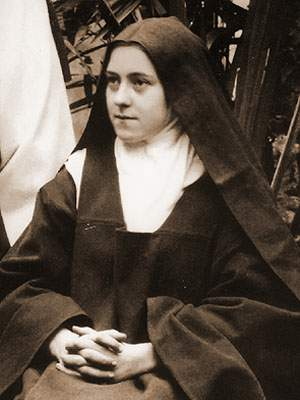
\includegraphics[scale=0.35]{theresia-2.jpg}
\end{center}
\end{floatingfigure}
Dalam autobiografinya, Theresia menyebutkan bahwa kesadaran ini mengawali kehidupannya yang baru, dimana Yesus telah menyembuhkannya dan menghilangkan sifat kepribadiannya yang buruk. Semenjak saat itu ia sadar bahwa dirinya dipenuhi oleh Roh Kudus, ia sadar bahwa ia harus mengabdikan seluruh hidupnya kepada Tuhan. Kerinduaanya untuk bersatu dengan kanak-kanak Yesus sangatlah besar dan oleh karena itulah dikemudian hari ia digelari "Santa Theresia dari Kanak-kanak Yesus". Kepada Yesus ia berjanji tidak akan pernah segan untuk melakukan apa saja yang dikehendaki Tuhan darinya. Betapa bahagia hati Theresia ketika pada umur 12 tahun ia boleh menyambut komuni untuk pertama kalinya. Dihadapan sebuah salib ia berjanji: "Yesus di kayu salib yang haus, saya akan memberikan air kepadaMu. Saya bersedia menderita sedapat mungkin agar banyak orang berdosa yang bertobat. Kerinduan Theresia yang begitu besar kepada Yesus mendesak ia untuk menjalani khusus sebagai biarawati mengikuti jejak ke 4 saudaranya yang lebih dahulu menjadi biarawati, namun ia belum bisa diterima di biara karena umurnya baru 14 tahun.

Pada umur 15 tahun saat berziarah ke Roma bersama ayahnya, Theresia dengan meminta izin khusus dari Bapa Suci agar ia diperkenankan menjadi biarawati. Permintaannya dikabulkan dan ia masuk diterima di lingkungan biara Carmelit di Lisieux Perancis.

Sembilan tahun lamanya ia hidup sebagai suster biasa, dan sebagaimana biasanya seorang suster muda, ia setiap hari melaksanakan tugas dan doa harian, harus mengatasi perasaan marah, tersinggung, iri hati, memerangi kebosanan dan berbagai ragam godaan lahir maupun batin. Untuk mencapai kesempurnaan hidup ia memilih "Jalan Sedehana" berdasarkan ajaran kitab suci yaitu hidup selaku anak kecil, penuh cinta dan iman akan kepercayaan Allah serta penyerahan diri yang total dengan penuh perasaan gembira. Demi cita-cita itu ia melakukan hal-hal kecil dan kewajiban sehari-hari di biara dengan penuh tanggung jawab karena cinta kasihnya yang besar kepada Allah Bapa di surga.

Ia sedih sekali melihat banyak orang menyakiti hati Yesus dengan berbuat dosa dan tidak mau bertobat. Untuk mempertobatkan orang-orang berdosa itu, ia mempersembahkan dirinya sebagai korban pepulih dosa-dosa. Ia rajin berdoa dan melakukan tapa bagi semua orang berdosa. Ia juga berdoa bagi para missionaris dan kemajuan kerajaan Allah di seluruh dunia.

Theresia akhirnya menderita sakit paru-paru yang sangat parah. Selama 2 tahun ia menanggung beban penderitaan itu dengan gembira. Penyakit ini kemudian merenggut nyawanya pada tanggal 30 September 1897 di biara Lisieux. Sebelum menghembuskan nafasnya ia berjanji untuk menurunkan hujan mawar ke dunia. Janji ini terpenuhi dengan banyaknya karunia Allah yang diberikan kepada semua orang yang berdoa dengan perantaranya. Theresia meninggal dalam usia yang sangat muda 24 tahun. Pada tahun 1925 ia ditetapkan sebagai "Santa" oleh Paus Pius XI (1922-1939) dan diangkat menjadi Santa pelindung negara Perancis oleh Paus Pius XII (1939-1958)

\subsubsection*{Setelah Theresia Wafat}

\begin{floatingfigure}[l]{2.75cm}
	\begin{center}
		\includegraphics[scale=0.275]{theresia-3.jpg}
	\end{center}
\end{floatingfigure}
Setelah wafat, Theresia menjadi terkenal karena buku yang ditulisnya "Kisah Suatu Jiwa," yang diterbitkan satu tahun setelah wafatnya (di Indonesia diterjemahkan dengan judul: 'Aku Percaya akan Cinta Kasih Allah'). Theresia dikanonisasi pada tahun 1925 oleh Paus Pius X. Ia dikenal dengan sebutan Santa Theresia dari Kanak-kanak Yesus atau Santa Theresia si Bunga Kecil. St. Theresia bersama-sama dengan St. Jeanne d'Arc diberi gelar Pelindung Perancis. Selain itu St. Theresia bersama-sama dengan St. Fransiskus Xaverius diberi gelar Pelindung Misionaris.  Pada tanggal 19 Oktober 1997, Theresia juga menjadi wanita ke-3 yang diberi gelar Doktor Gereja. Kita dapat mohon bantuannya mengenai apa saja. Ia pernah berjanji  akan melimpahi kita dengan bunga-bunga mawar dari surga dan memang, sejak kematiannya banyak mukjizat yang terjadi berkat bantuan doanya. Pestanya dirayakan setiap tanggal 1 Oktober.

\subsection*{Rahasia Theresia: Jalan Kecil, Jalan Kanak-Kanak Rohani}

Theresia seorang gadis yang sederhana dengan `jalan kecilnya' yang istimewa.  Ia menunjukkan bahwa \textbf{kekudusan dapat dicapai oleh siapa saja betapa pun rendah, hina dan biasanya orang itu}. Caranya ialah dengan melaksanakan pekerjaan-pekerjaan kecil dan tugas sehari-hari dengan penuh cinta kasih murni kepada Tuhan. Kamu pun dapat menjadi kudus dengan cara-cara sederhana seperti yang dilakukan oleh St. Theresia dengan jalan kecilnya.


\chapter{Data Umat Lingkungan}
\section{Daftar Umat pada tahun \tahun}
% \begin{longtable}{|m{5mm}|m{45mm}|m{20mm}|m{20mm}|C{10mm}|m{20mm}|m{20mm}|} 
\hline  
\multicolumn{1}{|c|}{\multirow{2}{*}{\textbf{No}}} & \multicolumn{1}{|c|}{\multirow{2}{*}{\textbf{Nama}}} & \multicolumn{2}{|c|}{\textbf{Lahir}} & 
\multicolumn{1}{|c|}{\multirow{2}{*}{\textbf{L/P}}}&
	\multicolumn{2}{|c|}{\textbf{Baptis}}  \\ \cline{3-4}\cline{6-7}
&&
\multicolumn{1}{|c|}{\textbf{Tempat}} & \multicolumn{1}{|c|}{\textbf{tanggal}} &
&
 \multicolumn{1}{|c|}{\textbf{Tempat}} & \multicolumn{1}{|c|}{\textbf{tanggal}} \\ 
\hline \hline  \endfirsthead 
\hline  
\multicolumn{1}{|c|}{\multirow{2}{*}{\textbf{No}}} & \multicolumn{1}{|c|}{\multirow{2}{*}{\textbf{Nama}}} & \multicolumn{2}{|c|}{\textbf{Lahir}} & 
\multicolumn{1}{|c|}{\multirow{2}{*}{\textbf{L/P}}}& \multicolumn{2}{|c|}{\textbf{Baptis}}  \\ \cline{3-4}\cline{6-7}
&&
\multicolumn{1}{|c|}{\textbf{Tempat}} & \multicolumn{1}{|c|}{\textbf{tanggal}} &
&
\multicolumn{1}{|c|}{\textbf{Tempat}} & \multicolumn{1}{|c|}{\textbf{tanggal}} \\ 
\hline \hline \endhead \endfoot
\newpage
\section{Data Umat}
\begin{center}
DATA UMAT LINGKUNGAN SANTO PETRUS\\
\end{center}
\scriptsize
\begin{longtable}{|r|l|l|p{1.7cm}|r|r|r|p{0.7cm}|}
99	&Y.B Sudibyo Martopangarso	&Sombomerten	&1234567890123&8	&8	&22	&AB/A\\ \kill
\hline
NO	&Nama Kepala	&A l a m a t / Blok	&Telephone	&\multicolumn{3}{|c|}{Aggt Kel.}&Gol\\ \cline{5-7}
	&Keluarga	&	&H.P	&L	&P	&Jml	&Drh\\
\hline
\endfirsthead
\hline
NO	&Nama Kepala	&A l a m a t	&Telephone	&\multicolumn{3}{|c|}{Aggt Kel.}&Gol\\ \cline{5-7}
	&Keluarga	&	&H.P	&L	&P	&Jml	&Drh\\
\hline
\endhead
1	&Yakobus Lasiman	&Sanggrahan	&08170426162	&3	&2	&5	&B/-\\
2	&Ignatius Saman	&Sanggrahan	&081578085478	&2	&2	&4	&A/O\\
3	&F.Noer Susilo Hartono	&Sanggrahan	&0274-7483220	&2	&2	&4	&O/O\\
4	&Yohanes Kamari	&Sanggrahan	&081342612992	&2	&3	&5	&O/O\\
5	&Th. Sri Budiati	&Kr. Nongko	&7480130	&	&1	&1	&\\
6	&A. Sudarmini (Bu Titus)	&Kr. Nongko	&0811267658, 4333604	&1	&1	&2	&\\
7	&Yosaphat Sugiyatno	&Kr. Nongko	&0811256059	&4	&2	&6	&AB/A\\
8	&A.M.Z. Sidhi Hastjarjo	&Kr. Nongko	&4333630	&1	&	&1	&A\\
9	&A.Y.Hery Purnomo	&Kr. Nongko	&4333515, 081328200141	&2	&2	&4	&AB/B\\
10	&Y.Z.Budiman Susanto	&Kr. Nongko	&4333578, 7471197, 08122942583	&3	&1	&4	&O/O\\
11	&R.F.H. Soegijono	&Kr. Nongko	&4333825	&3	&2	&5	&B/A\\
12	&Mateus Daryanto	&Kr. Nongko	&7892789	&1	&	&1	&\\
13	&Ibu Eko/ Th. Herlinawati	&Kr. Nongko	&7435255	&	&2	&2	&\\
14	&Robertus Susilo	&Kr. Nongko	&0274-7483220&1&1&2&O/O\\
15	&Hieronimous Subagyo	&Kr. Nongko	&4333584	&2	&2	&	&\\
16 &Stefanus Subagyo &Kr. Nongko &081328080811& & & &\\
17	&Theodorus Totok Suyanto	&Kr. Nongko	&081392025525	&	&	&	&\\
18	&B.N.Sami Raharja	&Pugeran	&4333807, 081578778777	&2	&3	&5	&A/O\\
19	&M.M. Sri Pramuwati	&Pugeran	&4333807	&1	&1	&2	&\\
20	&Y.B Sudibyo Martopangarso	&Pugeran	&7496866, 08164229555, 4333829	&1	&1	&2	&\\
21	&Y.Sudarmadi/Serly	&Pugeran	&4333545, 081578898484	&2	&2	&4	&O/O\\
22 & FX Aris Wibowo S & Pugeran &085867335678 & 1 & 1 & 2 & O/B\\
23	&Aloysius Lamakey	&Pugeran	&4333684, 085643173281	&2	&3	&5	&A/AB\\
24	&Yakobus Nina Lamakey	&Pugeran	&7839098	&2	&1	&3	&\\
25	&Yohanes Suripto	&Pugeran	&4333820, 0817889303	&4	&1	&5	&\\
26	&Neo Suradi	&Pugeran	&556180, 081578115615	&1	&2	&3	&B/O\\
27	&A.Waldiman	&Pugeran	&	&3	&2	&5	&A/O\\
28	&A.Sujarwanto	&Pugeran	&4333577, 085643430434	&2	&3	&5	&AB/O\\
29	&C.S. Prihatiningtyas Purwadi	&Pugeran	&7440441, 7400625, 08122940457	&1	&2	&3	&O/A\\
30	&C.Supriyadi	&Pugeran	&4333884, 081328450101	&2	&2	&4	&A/-\\
31	&Thomas Baharudin (Mia)	&Pugeran	&085253890448	&1	&2	&3	&A/\\
32	&Andreas Keso Muda	&Pugeran	&081328692102	&1	&3	&4	&A/B\\
33	&Paulus Suroyo	&Pugeran	&4333667, 08122752803	&2	&2	&4	&\\
34	&Fx Sularto	&Pugeran	&081314190698	&1	&1	&2	&\\
35	&Petrus Samino	&Pugeran	&	&1	&1	&2	&\\
36 &Domi Sukanto &Pugeran & & & & &\\
37 &Agustinus Sumaryono&Maguwo Asri&081804264250&1&0&1&B\\
38	&Yohanes Suyanto	&Sombomerten	&4333886, 08562869037	&4	&2	&6	&B/A\\
39	&M.Theresia Nanik Ismarjiati	&Sombomerten	&4333892, 08156861272	&2	&1	&3	&O/O\\
40	&Ign. Luddy Indra P.	&Maguwo	&4333648, 08122700806	&2	&2	&4	&O/O\\
41	&Y.B. Kandari	&Nanggulan 	&	&1	&	&1	&O\\
42	&Y.F.Lina Setyaningsih	&Nanggulan 	&08157966006	&1	&2	&3	&B/O\\
43	&N. Putut Andoko	&Nanggulan 	&085221610549	&1	&3	&4	&\\
44	&S.Rumiyati Siswanto	&Nanggulan 	&081328217018	&	&2	&2	&\\
45	&A.Dwi Wahyuni (Nunik)	&Nanggulan 	&081392704876	&1	&2	&3	&O/A\\
46	&C. Srimurhariyani Sudarto	&Nanggulan 	&486955, 081328000523	&1	&3	&4	&A\\
47	&Ign. Mulyono	&Nanggulan 	&484617	&1	&1	&2	&O\\
48	&V. Sugiyati	&Nanggulan 	&488074	&1	&1	&2	&B\\
49	&R.Abbas Suhardjo	&Nanggulan 	&485671, 081328564524	&1	&1	&2	&AB/A\\
50	&Y. Laba Atawolo	&Nanggulan 	&08122745350	&1	&1	&2	&B/B\\
51	&Ch.Sri Supartiningsih	&Nanggulan 	&08122983365	&1	&	&1	&O\\
52	&Agung Danan Jaya	&Nanggulan 	&085228245479	&2	&1	&3	&\\
53	&Ign. Ardi Subardi	&Nanggulan 	&4333865	&2	&1	&3	&B/A\\
54	&Thomas Sukijo	&Nanggulan 	&487164, 0817267423	&1	&1	&2	&B\\
55	&Agus/Wiwid	&Nanggulan 	&487164	&1	&3	&4	&B\\
56	&A. Winarso	&Nanggulan 	&0816675362	&3	&2	&5	&\\
57	&Albertus Purwoto	&Nanggulan 	&0818468374	&1	&3	&4	&\\
58	&M.Supangat	&Nanggulan 	&081578043761, 081802794742	&2	&3	&5	&O/B\\
59	&C.Hendro Muryanto	&Nanggulan 	&081328032468	&2	&1	&3	&\\
60	&C.Supartiyah (Bu Tris)	&Nanggulan 	&085228928010	&1	&1	&2	&O\\
61	&Y.Eko Hananto	&Nanggulan 	&081392258790	&2	&1	&3	&\\
62	&V.Ratnasih A. Sukiyanto	&Kembang	&488326, 08562907933	&1	&1	&2	&O\\
63	&D.Damar Dwi Nugroho	&Kembang	&488326, 08132836667	&2	&1	&3	&O/O\\ \hline
	&	&	&	&94	&96	&186	&\\ \hline
	\multicolumn{7}{l}{NB: Revisi data harap hubungi ketua/sekretaris lingkungan}\\
%% 	&	&	&	&	&	&	&\\
%% 	&	&	&	&	&	&	&\\
%% 	&	&	&	&	&	&	&\\
%% 	&PINDAH	&	&	&	&	&	&\\
%% 1	&Y. Bejo Praptohardjono	&Nanggulan 	&Bergabung dg KK Bu Nunik	&2	&	&	&\\
%% 2	&Suranto	&Nanggulan 	&Bergabung dg KK Bu Lina	&1	&	&	&\\
%% 3	&Kunto	&Maguwo	&Pindah bulan April 2007	&	&	&0	&\\
%% 4	&H. Endro Cahyono	&Nanggulan 	&08164221960	&2	&1	&3	&\\
%% 	&	&	&	&	&	&	&\\
%% 	&Penambahan	&	&	&	&	&	&\\
%% 1	&C.Hendro Muryanto	&Nanggulan 	&Pemecahan KK dg Bu Tris	&2	&1	&3	&\\
%% 2	&Sutrino	&Pugeran	&Umat Baru 03/01/2007	&	&	&4	&\\
%% 3	&M.M. Sri Pramuwati	&Pugeran	&Pecah KK dg bpk. Sami Rahardjo	&1	&1	&2	&\\
%% 4	&Robertus Susilo	&Sanggrahan	&Pecah KK dg bpk. F.Noer Susilo	&1	&1	&2	&\\
%% 5	&Mateus Daryanto	&Karang Nongko	&Umat Baru 22/02/2007	&2	&	&2	&\\
%% 6	&Ibu Christina Dina	&Sanggrahan	&Calon ybs belum ketemu	&	&1	&1	&\\
%% 7	&Ibu Eko	&Karang Nongko	&ybs ok 22/02/07	&	&2	&2	&\\
%% 8	&Tri Mastoyo Jati Kesuma	&Pugeran	&4333590 (Isteri belum mau gabung)	&	&	&0	&\\
%% 9	&Theresia Sri Budiarti	&Karang Nongko	&Warga baru 30/06/07	&	&1	&1	&\\
%% 10	&Yoseph Hary	&Kembang	&Warga baru 16/06/07, telp.487667	&2	&1	&3	&\\
%% 11	&Ida	&Pugeran	&Warga baru 01/05/07	&1	&1	&2	&\\
%% 12	&Y.Eko Hananto	&Nanggulan 	&Warga lama pindah kembali	&2	&1	&3	&\\
%% 13	&Y. Djoko Marsito	&Pugeran	&Warga baru 27/10/06	&2	&1	&3	&\\
%% 14	&Kaldinus Benedictus Diler	&Sanggrahan	&Warga baru 14/05/07	&1	&1	&2	&\\

\end{longtable}
\normalsize

\section[Daftar keluarga]{Daftar Keluarga yang senyatanya berdomisili di lingkungan pada tahun \tahun}
% \begin{longtable}{|l|l|m{59mm}|C{15mm}|C{15mm}|} 
\hline \multicolumn{1}{|c|}{\multirow{2}{*}{\textbf{No}}} & \multicolumn{1}{|c|}{\multirow{2}{*}{\textbf{Np}}} & \multicolumn{1}{|c|}{\multirow{2}{*}{\textbf{Nama}}} & \multicolumn{2}{|c|}{\textbf{Domisili}} \\ \cline{4-5}
&&&Ya&Tidak \\ \hline \hline
  \endfirsthead 

\hline \multicolumn{1}{|c|}{\multirow{2}{*}{\textbf{No}}} & \multicolumn{1}{|c|}{\multirow{2}{*}{\textbf{Np}}} & \multicolumn{1}{|c|}{\multirow{2}{*}{\textbf{Nama}}} & \multicolumn{2}{|c|}{\textbf{Domisili}} \\ \cline{4-5}
&&&Ya&Tidak \\ \hline \hline
\endhead \endfoot

 \begin{longtable}{|l|l|m{59mm}|C{15mm}|C{15mm}|} 
	\hline \multicolumn{1}{|c|}{\multirow{2}{*}{\textbf{No}}} 
	& \multicolumn{1}{|c|}{\multirow{2}{*}{\textbf{Np}}} & \multicolumn{1}{|c|}{\multirow{2}{*}{\textbf{Nama}}} 
	& \multicolumn{2}{|c|}{\textbf{Domisili}} \\ \cline{4-5}
	&&&Ya&Tidak \\ \hline \hline
	\endfirsthead 
	
	\hline \multicolumn{1}{|c|}{\multirow{2}{*}{\textbf{No}}} & \multicolumn{1}{|c|}{\multirow{2}{*}{\textbf{Np}}} 
	& \multicolumn{1}{|c|}{\multirow{2}{*}{\textbf{Nama}}} & \multicolumn{2}{|c|}{\textbf{Domisili}} \\ \cline{4-5}
	&&&Ya&Tidak \\ \hline \hline
	\endhead \endfoot
	
	1&30016015210009&Sunaryo Prononagoro Kra, Yohanes Pemandi&Ya&\\ \hline 
	2&30016015210455&Ariwibowo Sudaryanto, Fransiskus Xaverius&Ya&\\ \hline 
	3&30016015210458&Saptanto Sarwo Basuki, Yohanes&&Tidak\\ \hline 
	4&30016015210033&Triyono, Cornelius&Ya&\\ \hline 
	5&30016015210001&Banarudin, Thomas&Ya&\\ \hline 
	6&30016015210002&Keso Muda, Andreas&Ya&\\ \hline 
	7&30016015210003&Aloysius Lamakey&Ya&\\ \hline 
	8&30016015210004&Mardi Susanti, Agustina&Ya&\\ \hline 
	9&30016015210005&Nanik Ismarjati, Maria Theresia&Ya&\\ \hline 
	10&30016015210007&Temon Siswo Utomo, Margaretha&Ya&\\ \hline 
	11&30016015210008&Sandi Ignatius&Ya&\\ \hline 
	12&30016015210010&Sudarmadi, Yohanes&Ya&\\ \hline 
	13&30016015210011&Sujarwanto, Agustinus&&Tidak\\ \hline 
	14&30016015210013&Sularto, Fransiscus Xaverius&Ya&\\ \hline 
	15&30016015210014&Supriadi, Cornelius&Ya&\\ \hline 
	16&30016015210435&Krisni Prihartati, Cornelia&&Tidak\\ \hline 
	17&30016015210015&Suradi, Neo&Ya&\\ \hline 
	18&30016015210016&Suroyo, Paulus&Ya&\\ \hline 
	19&30016015210017&Suyanto, Yohanes&Ya&\\ \hline 
	20&30016015210018&Suprihatin, Kristina&Ya&\\ \hline 
	21&30016015210021&Niha Lamakey, Yakobus&Ya&\\ \hline 
	22&30016015210022&Suripto, Yohanes&Ya&\\ \hline 
	23&30016015210437&Setyawan Putra, Thomas&Ya&\\ \hline 
	24&30016015210439&Dalyono, Valentinus&Ya&\\ \hline 
	25&30016015210440&Supriyana, Antonius&Ya&\\ \hline 
	26&30016015210451&Djoko Marsito, Yohanes&Ya&\\ \hline 
	27&30016015210452&Heru Pratomo, Aloysius&Ya&\\ \hline 
	28&30016015210459&Gelungminangkoro Widyanurcahyo, Dominikus&Ya&\\ \hline 
	&Total & &25&3\\ \hline 
\end{longtable}

\chapter{Penambahan Umat Tahun \tahun}
\section{Penambahan umat melalui sakramen inisiasi dan pengukuhan}
 \begin{longtable}{|r|l|r@{$-$}l|r|} 
	\caption*{Data rekap} \\
	\hline \multicolumn{1}{|c|}{\textbf{No.}} & 
	\multicolumn{1}{|c|}{\textbf{Baptis/Pengukuhan}} &
	\multicolumn{2}{c}{\textbf{Umur}} & \multicolumn{1}{|c|}{\textbf{Jumlah}} \\
	\hline \hline  \endfirsthead 
	
	1&Bayi&0&4&1\\ \hline 
	2&Anak&5&10&0\\ \hline 
	3&Remaja&11&16&0\\ \hline 
	4&Dewasa&17&&0\\ \hline 
	5&Pengukuhan (dari Kristen Prostestan)&& &0\\ \hline 
	6&Jumlah&&&1\\ \hline 
\end{longtable}


\begin{longtable}{|l|m{60mm}|l|l|l|}
	\caption*{Data detail} \\
	\hline \hline 
	\multicolumn{1}{|c|}{\textbf{No}} & 
	\multicolumn{1}{|c|}{\textbf{Nama}} & 
	\multicolumn{1}{|c|}{\textbf{Tgl lahir}} &
	\multicolumn{1}{|c|}{\textbf{Tgl baptis}} &
	\multicolumn{1}{|c|}{\textbf{Kelompok}} 
	\\ \hline \hline  
	\endfirsthead
	
	1&Cintakirana Achiera, Gabrielle&2015-11-10&2016-01-10&Bayi\\ \hline 
\end{longtable}

\section[Penambahan umat \dots]{Penambahan umat melalui mutasi dari lingkungan/wilayah/stasi/paroki/keuskupan lain}
 \begin{longtable}{|p{0.5cm}|l|r|} 
	\caption*{Data rekap} \\
	\hline 	\hline 
	\multicolumn{1}{|c|}{\textbf{No}} & 
	\multicolumn{1}{|c|}{\textbf{Jenis Mutasi}} & \multicolumn{1}{|c|}{\textbf{Jumlah}} \\ \hline \hline  \endfirsthead
	\hline \hline \endfoot 
	
	1&Pindah Keuskupan&5\\ \hline 
	2&Pindah Lingkungan&0\\ \hline 
	3&Pindah Paroki&3\\ \hline 
	4&Pindah Wilayah&0\\ \hline 
	5&Jumlah&9\\ \hline 
\end{longtable}



\begin{longtable}{|l|m{6cm}|C{25mm}|l|}
	\caption*{Data detail} \\
	\hline \hline 
	\multicolumn{1}{|c|}{\textbf{No}} & 
	\multicolumn{1}{|c|}{\textbf{Nama}} & 
	\multicolumn{1}{|c|}{\textbf{Tahun masuk}} &
	\multicolumn{1}{|c|}{\textbf{Mutasi}}  
	\\ \hline \hline  
	\endfirsthead
	\hline 
	\endfoot
	\hline \hline 
	\multicolumn{1}{|c|}{\textbf{No}} & 
	\multicolumn{1}{|c|}{\textbf{Nama}} & 
	\multicolumn{1}{|c|}{\textbf{Tahun masuk}} &
	\multicolumn{1}{|c|}{\textbf{Mutasi}}  
	\\ \hline \hline  
	\endhead
	
	1&Cintakirana Achiera, Gabrielle&2016&Pindah Paroki\\ \hline 
	2&Vania Melianta, Aquilina &2016&Pindah Paroki\\ \hline 
	3&Gelungminangkoro Widyanurcahyo, Dominikus&2016&Pindah Paroki\\ \hline 
	4&Isti Rudati, Valentina&2016&Pindah Keuskupan\\ \hline 
	5&Desicea Calista, Redempta&2016&Pindah Keuskupan\\ \hline 
	6&Saptanto Sarwo Basuki, Yohanes&2016&Pindah Keuskupan\\ \hline 
	7&Hargyan Revano, Petrus Krisologus&2016&Pindah Keuskupan\\ \hline 
	8&Stanley Andi Pradana, Ignatius&2016&Pindah Keuskupan\\ \hline 
\end{longtable}

\chapter{Pengurangan Umat}
 \begin{longtable}{|l|l|r|} 
	\hline \endhead \hline \endfoot \hline 
	\hline 
	\multicolumn{1}{|c|}{\textbf{No}} & 
	\multicolumn{1}{|c|}{\textbf{Alasan}} & \multicolumn{1}{|c|}{\textbf{Jumlah}} \\ \hline \hline  \endfirsthead
	
	1&Meninggal Dunia&1\\ \hline 
	2&Pindah Lingkungan&0\\ \hline 
	3&Pindah Agama&0\\ \hline 
	4&Jumlah&1\\ \hline 
\end{longtable}


\begin{longtable}{|l|m{6cm}|C{25mm}|l|}
	\caption*{Data detail} \\
	\hline \hline 
	\multicolumn{1}{|c|}{\textbf{No}} & 
	\multicolumn{1}{|c|}{\textbf{Nama}} & 
	\multicolumn{1}{|c|}{\textbf{Tgl Mutasi}} &
	\multicolumn{1}{|c|}{\textbf{Mutasi}}  
	\\ \hline \hline  
	\endfirsthead
	\hline 
	\endfoot
	\hline \hline 
	\multicolumn{1}{|c|}{\textbf{No}} & 
	\multicolumn{1}{|c|}{\textbf{Nama}} & 
	\multicolumn{1}{|c|}{\textbf{Tgl Mutasi}} &
	\multicolumn{1}{|c|}{\textbf{Mutasi}}  
	\\ \hline \hline  
	\endhead
	
	1&Suci Wahyuningsih, Theresia&2016-10-10&Meninggal Dunia\\ \hline 
\end{longtable}

\chapter{Calon Biarawan/Biarawati}
 \begin{longtable}{|r|l|l|l|l|l|} 
	\hline \hline 
	\multicolumn{1}{|c|}{\textbf{No}} & 
	\multicolumn{1}{|c|}{\textbf{Nama calon}} & 
	\multicolumn{3}{|c|}{\textbf{Biarawan/wati}} & 
	\multicolumn{1}{|c|}{\textbf{Nama orang tua/ wali}} \\ \cline{3-5}  
	&& \multicolumn{1}{|c|}{\textbf{Imam}} & 
	\multicolumn{1}{|c|}{\textbf{Bruder}} &  \multicolumn{1}{|c|}{\textbf{Suster}} & 
	\\  
	\hline \hline  \endfirsthead
1 &  & & & & \\ \hline 
2 &  & & & & \\ \hline 
3 &  & & & & \\ \hline 
\end{longtable}


\chapter{Penerimaan Sakramen}
 \begin{longtable}{|l|l|r|}
	\caption*{Data rekap} \\
	\hline \hline 
	\hline 
	\multicolumn{1}{|c|}{\textbf{No}} & 
	\multicolumn{1}{|c|}{\textbf{Sakramen}} & \multicolumn{1}{|c|}{\textbf{Jumlah}} \\ \hline \hline  
	\endfirsthead
	
	1&Komuni Pertama&0\\ \hline 
	2&Penguatan&4\\ \hline 
	3&Perkawinan&0\\ \hline 
	4&Pengurapan Orang Sakit&0\\ \hline 
	5&Jumlah&4\\ \hline 
\end{longtable}



\begin{longtable}{|l|m{6cm}|C{25mm}|l|}
	\caption*{Data detail} \\
	\hline \hline 
	\multicolumn{1}{|c|}{\textbf{No}} & 
	\multicolumn{1}{|c|}{\textbf{Nama}} & 
	\multicolumn{1}{|c|}{\textbf{Tangal}} &
	\multicolumn{1}{|c|}{\textbf{Sakramen}}  
	\\ \hline \hline  
	\endfirsthead
	\hline 
	\endfoot
	\hline \hline 
	\multicolumn{1}{|c|}{\textbf{No}} & 
	\multicolumn{1}{|c|}{\textbf{Nama}} & 
	\multicolumn{1}{|c|}{\textbf{Tangal}} &
	\multicolumn{1}{|c|}{\textbf{Sakramen}}  
	\\ \hline \hline  
	\endhead
	
	1&Triyono, Cornelius&2016-10-09&Penguatan\\ \hline 
	2&Apriliana Wulandari, Herminigilda&2016-10-09&Penguatan\\ \hline 
	3&Oldi Kristianto, Eduardus&2016-10-09&Penguatan\\ \hline 
	4&Gelungminangkoro Widyanurcahyo, Dominikus&2016-10-09&Penguatan\\ \hline 
\end{longtable}

\chapter{Peristiwa-peristiwa Penting}
\begin{table}[h!]
\centering
\begin{tabular}{|l|l|r|l|}
	\hline
	\textbf{No}&\textbf{Peristiwa-peristiwa penting}&\textbf{Tanggal}&\textbf{Tempat}\\ \hline
	1.&Natalan lingkungan & 6-Jan-2016 & Joglo Lawas\\ \hline
	2.&Paskahan lingkungan & 7-Apr-2016 & Joglo Lawas\\ \hline
	3.&Ziarah lingkungan & 28-Mei-2016 & Sendang Jatiningsih \\ \hline
	4.&Pesta nama & 31-Okt-2016 & Joglo Lawas \\ \hline 
	5.&Pemilihan pengurus baru& 10-Nov-2016 & Neo Suradi\\ \hline
\end{tabular}
\end{table}

\end{document}